\chapter{Projeto: ncRNA-Agents}
\label{sec:propostaNcRNAs}

Neste capítulo, apresentamos a arquitetura de um sistema de anota\c{c}\~ao de ncRNAs baseado em SMAs. Na Se\c{c}\~ao \ref{sec:ArqAnotacao}, apresentaremos a arquitetura adotada no sistema ncRNA-Agents. Na Se\c{c}\~ao \ref{sec:Implemetacao}, serão apresentandos os detalhes da implementa\c{c}\~ao do ncRNA-Agents.


\subsection{Arquitetura} \label{sec:ArqAnotacao}

Observamos que o presente projeto foi inspirado no trabalho de Ralha e 
co-autores~\citep{Schneider2006:2006,Ralha2011:2011}, que propuseram um sistema para anotação baseado em SMAs, denominado BioAgents Figura \ref{fig:441}.

\begin{landscape}
\begin{figure}[htb!]
\centering
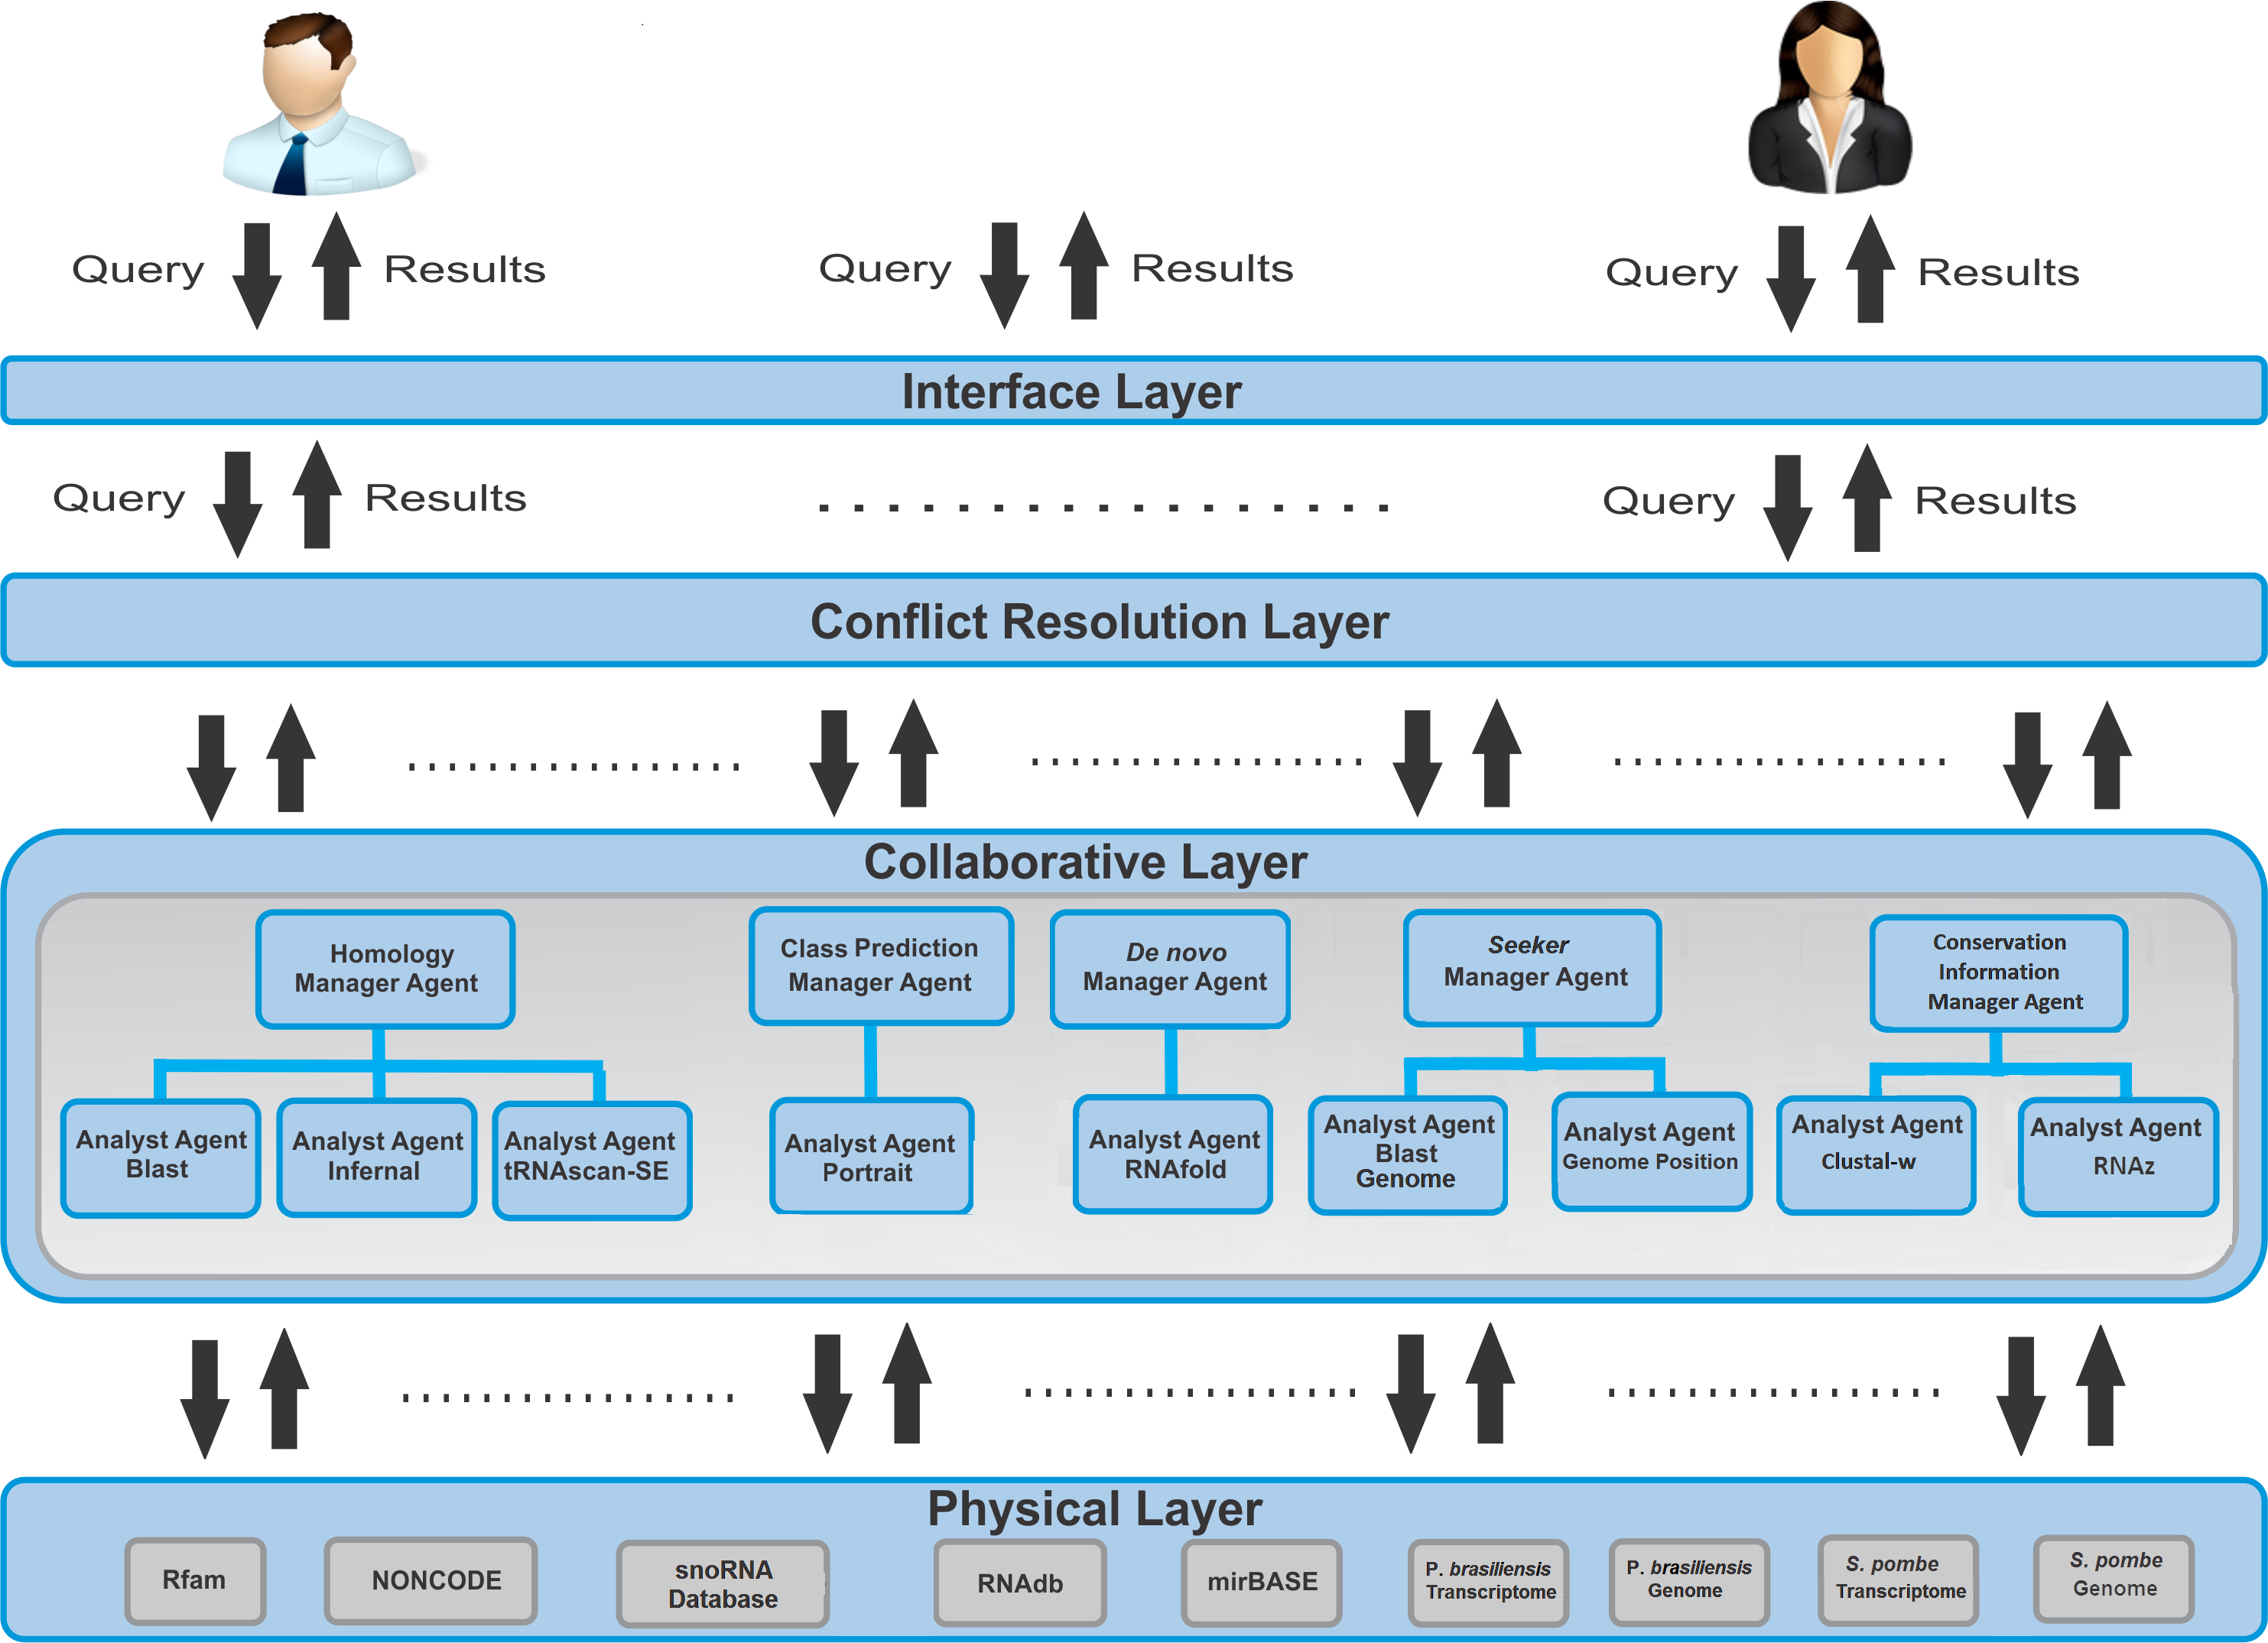
\includegraphics[angle=0,width=1.4\textwidth]{imagens//Arquitetura2sem1.png}
\caption{Arquitetura do ncRNAs-Agents.~\citep{Arruda:2011}. 
\label{fig:441}}
\end{figure}
\end{landscape}


\subsubsection{Descri\c{c}\~ao das Camadas} \label{sec:DescriCamada}

A \textbf{camada de interface} recebe a requisi\c{c}\~ao do usu\'ario composta por um arquivo com sequ\^encias em formato FASTA e indica\c{c}\~ao de ferramentas de anota\c{c}\~ao, e uma retorna os resultados de anota\c{c}\~ao das sequ\^encias de ncRNAs para o usu\'ario. A \textbf{camada de resolu\c{c}\~ao de conflitos} decide qual \'e a melhor recomenda\c{c}\~ao para a anota\c{c}\~ao de cada sequ\^encia recebida da camada de interface, a partir das diversas sugest\~oes recebidas da camada colaborativa, e informa essa decis\~ao para a camada de interface. A \textbf{camada colaborativa} \'e respons\'avel pela execu\c{c}\~ao das diversas ferramentas para identifica\c{c}\~ao e classifica\c{c}\~ao de ncRNAs, enviando os resultados obtidos para a camada de resolu\c{c}\~ao de conflitos. A \textbf{camada f\'isica} \'e formada por banco de dados.

\subsubsection{Descri\c{c}\~ao dos Agentes} \label{sec:DescriAgentes}

Na \textbf{camada colaborativa} existem dois tipos de agentes: \textbf{Agentes Gerentes} e \textbf{Agentes Analistas}. Os \textbf{Agentes Gerentes} realizam um filtro nas sugest\~oes enviadas pelos Agentes Analistas. Temos tr\^es tipos de Agentes Gerentes, conforme as tr\^es abordagens descritas na se\c{c}\~ao \ref{sec:Anotacao}. \textbf{Agente Gerente de Homologia} coordena agentes que trabalham com ferramentas baseadas em homologia. Dois exemplos s\~ao: (i) BLAST~\citep{altschul1990basic:1990}, que considera apenas a estrutura prim\'aria da sequ\^encia e identifica bem os snoRNAs~\citep{durbin1998biological:1998}; e (ii) Infernal~\citep{eddy2003infernal:2003}. O \textbf{Agente Gerente Predi\c{c}\~ao de Classe} coordena os agentes que trabalham com ferramentas baseadas em Aprendizagem de M\'aquina. Um exemplo \'e o SVM-Portrait~\citep{Arrial:2006}. O \textbf{Agente Gerente \textit{De novo}} gerencia agentes que trabalham com ferramentas que não usam organismos de refer\^encia. Um exemplo \'e o RNAz~\citep{washietl2005fast:2005}, do pacote do Vienna, baseados em modelo termodin\^amico. O \textbf{Agente Gerente Alinhamento} coordena agentes que trabalham com ferramentas de alinhamento, resultantes de métodos de comparação de sequência, com o intuito de descobrir motivos comuns ou regi\~oes que permitam verificar se a sequ\^encia \'e de fato um ncRNA.


Os \textbf{Agentes Analistas} s\~ao respons\'aveis por executar ferramentas espec\'ificas para identificar e classificar ncRNAs. Cada Agente Analista, criado por solicita\c{c}\~ao de um Agente Gerente, executa uma an\'alise (\textit{parse}) para extrair informa\c{c}\~oes do arquivo de sa\'ida criado pela ferramenta espec\'ifica controlada por ele. O resultado dessa an\'alise \'e retornado ao Agente Gerente solicitante como recomenda\c{c}\~ao de anota\c{c}\~ao.


\subsection{Detalhes de Implementa\c{c}\~ao} \label{sec:Implemetacao}

Como prova de conceito, foi implementado um prot\'otipo com tr\^es Agentes Gerentes e realizados dois experimentos. 

\subsubsection{Detalhes}


Foi utilizada a plataforma Jade, por diversos motivos: (i) ser distribu\'ido como software sob licen\c{c}a LGPL; (ii) a linguagem de programa\c{c}\~ao suportada ser Java, possibilitando portabilidade; (iii) as especifica\c{c}\~oes de JADE serem compat\'iveis com o padr\~ao FIPA, oferecendo uma biblioteca de classes de protocolos  de intera\c{c}\~ao padronizados e prontas para serem instanciadas; (iv) a disponibiliza\c{c}\~ao da plataforma de agentes, com funcionalidades e ontologia de agentes,  mecanismos transporte e parsing de mensagens; (v) oferece uma comunica\c{c}\~ao eficiente de mensagens entre os agentes com a linguagem ACL~\citep{fipa:2002}, (vi) possui suporte a usu\'arios, tendo uma comunidade grande e ativa de desenvolvedores e vasta documenta\c{c}\~ao dispon\'ivel para consulta.

Foi utilizado o Drools para simula\c{c}\~ao do racioc\'inio por meio de infer\^encias nos agentes, pois permite programar regras de neg\'ocio declarativamente, separar e centralizar as regras de neg\'ocio de um sistema, e gerenciar regras alterando-as dinamicamente.


\subsubsection{Resultados} \label{sec:ResultadosObtidos}

Para a validação do método proposto neste trabalho, foram realizados dois experimentos baseados no Projeto \textit{Paracoccidioides brasilienses} Genoma do (Projeto Genoma Pb) e no Projeto Genoma Guaraná. Ambos os experimentos foram executados tanto para validar o funcionamento do sistema quanto para verificar a acurácia da ferramenta.


A Figura~\ref{sec:Interface} mostra a tela inicial e as ferramentas e bancos de dados já instalados no ncRNA-Agents.

As Figuras \ref{sec:TelaRespostaInfernal} e \ref{sec:TelaFinalExec} mostram \textit{screenshots} de \textit{sniffers} para visualização do comportamento dos agentes do ncRNA-Agents

\begin{landscape}
\begin{figure}[htb!] 
\centering
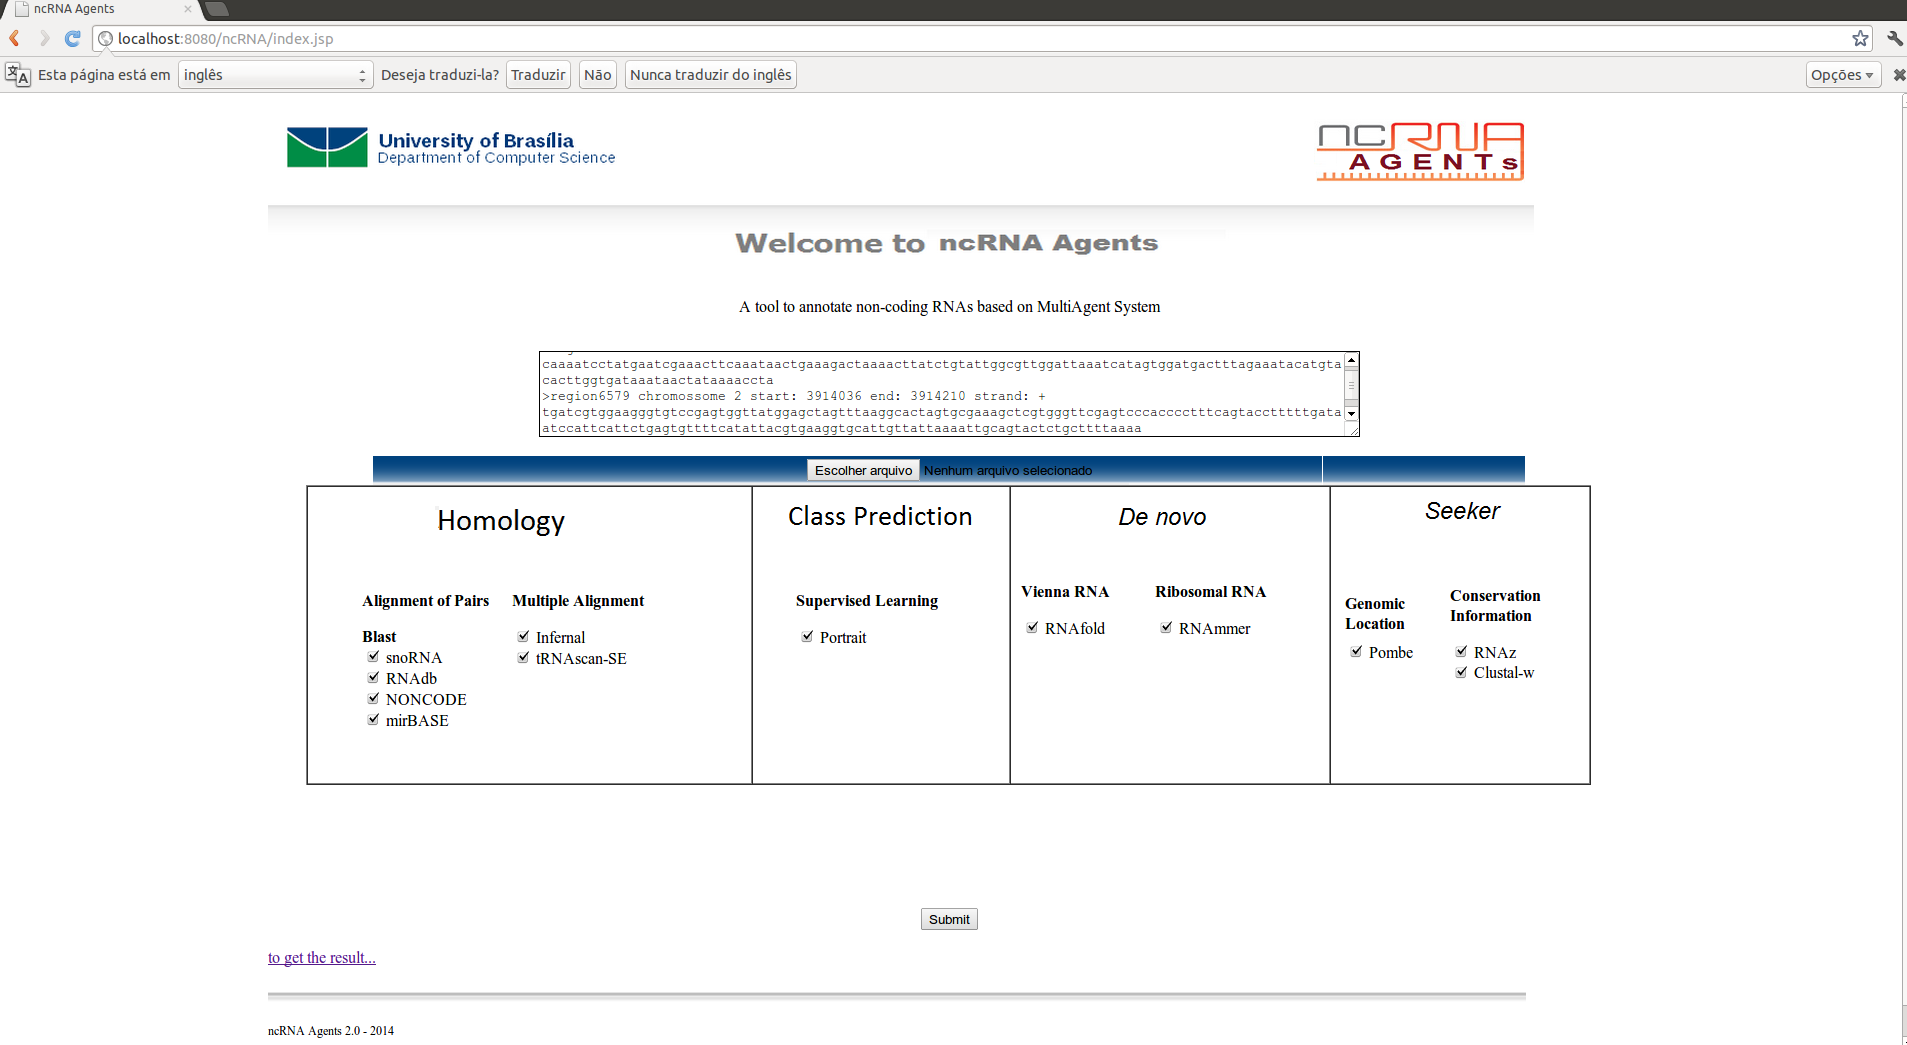
\includegraphics[angle=0,width=1.5\textwidth]{imagens//Interface.png}
\caption{Página do ncRNA-Agents, mostrando as ferramentas e os bancos de dados usados nos experimentos.} \label{sec:Interface}
\end{figure}
\end{landscape}

\begin{landscape}
\begin{figure}[htb!]
\centering
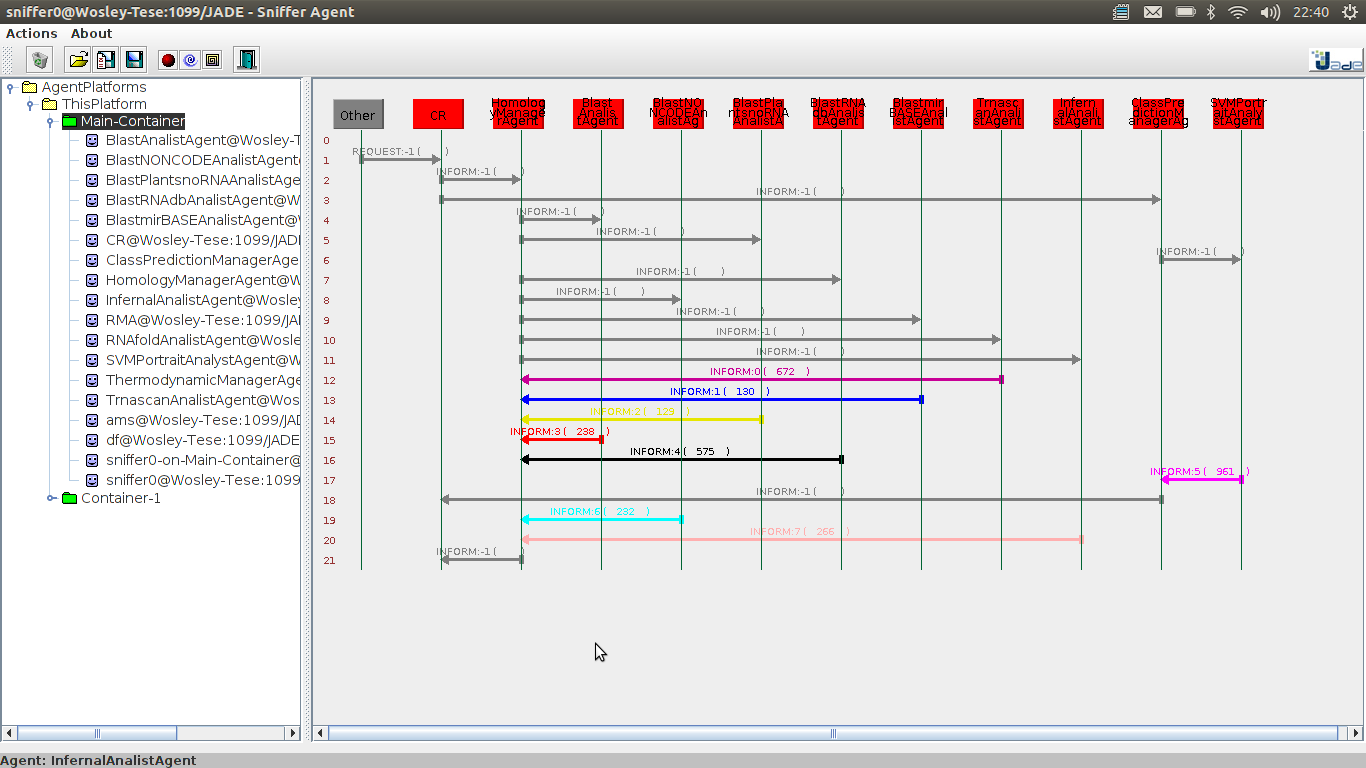
\includegraphics[angle=0,width=1.5\textwidth]{imagens//RespostaInferanal.png}
\caption{\textit{Sniffer} dos agentes do ncRNA-Agents: a camada de resolução de conflitos aguardando a resposta do Agente Gerente Homologia com a ferramenta Infernal.\label{sec:TelaRespostaInfernal}}
\end{figure}
\end{landscape}

\begin{landscape}
\begin{figure}[htb!]
\centering
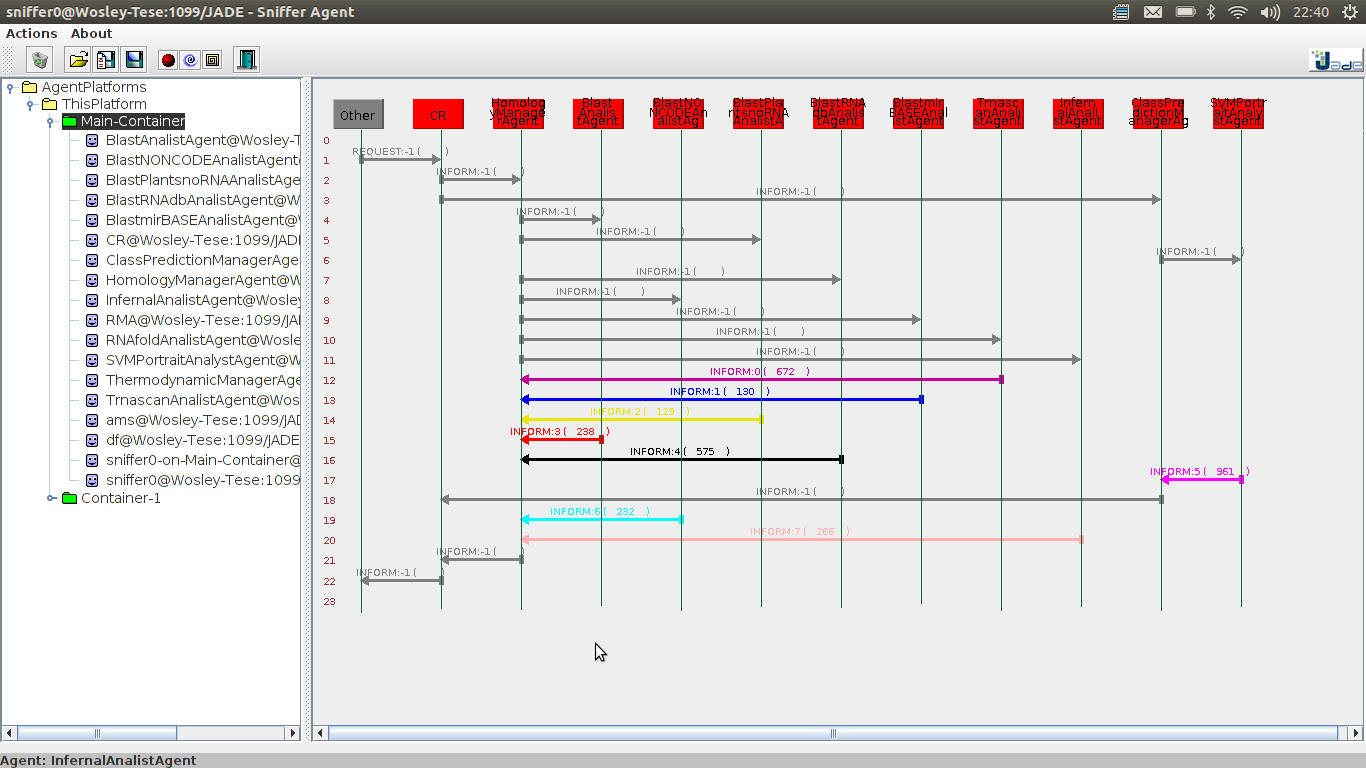
\includegraphics[angle=0,width=1.5\textwidth]{imagens//FinalExe.png}
\caption{\textit{Sniffer} dos agentes do ncRNA-Agents: a camada de resolução de conflitos enviando resposta para a interface do ncRNA-Agents para o usuário.\label{sec:TelaFinalExec}}
\end{figure}
\end{landscape}



\newpage
\subsubsection*{Obtidos} \label{sec:Resulobtidos}

Os estudos de caso foram conduzidos para identificar ncRNAs em dois projetos transcritoma: Projeto Genoma Pb e Projeto Genoma Guaraná. No primeiro, foram utilizados: o BLAST com os bancos de dados snoRNA, RNAdb, NONCODE, mirBASE, Infernal e o banco de Rfam 10.1, trRNAscan-SE e SVM-Portrait. No Projeto Genoma Guaraná, foram usados esses mesmos bancos, além do banco de dados Plant-snoRNA.

Esses estudos foram feitos utilizando 200 sequências de cada projeto, buscando a identificação de ncRNAs, observando-se que ainda não foram identificados ncRNAs nos dois projetos. As Tabelas~\ref{fig:ResulProjPb} e ~\ref{fig:ResulProjGuarana} mostram os resultados obtidos.


\begin{table}[htb!]
\caption{ncRNAs identificados no Projeto Genoma Pb.} \label{fig:ResulProjPb}
\centering
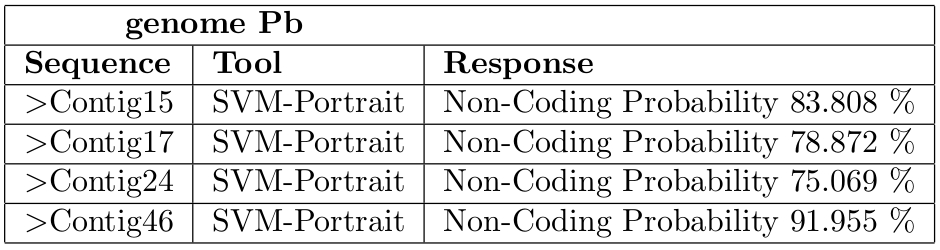
\includegraphics[angle=0,width=0.8\textwidth]{imagens//fig2.JPEG} %\label{fig:AcidosNucleicos}}
\end{table}


\begin{table}[htb!]
\caption{ncRNAs identificados no Projeto Genoma Guaraná.} \label{fig:ResulProjGuarana}
\centering
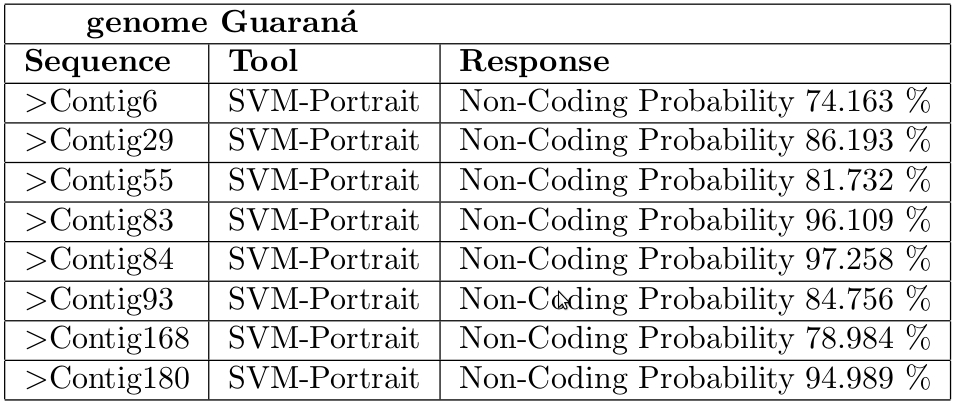
\includegraphics[angle=0,width=0.8\textwidth]{imagens//fig1.JPEG}
\end{table}

\subsubsection*{Esperados} \label{sec:Resulobter}

Os testes nos dois projetos serão estendidos para todas as sequências dos dois Projetos Genoma, Pb (6.022) sequências e Guaraná (8.613).
